\documentclass[a4paper,12pt]{article}
\usepackage[a4paper, top=2cm, bottom=2cm]{geometry}
\usepackage{amsmath}
\usepackage{amssymb}
\usepackage[utf8]{inputenc}
% \usepackage[T1]{fontenc}
\usepackage[vietnamese]{babel}
\usepackage[utf8]{vietnam}
\usepackage{xcolor}
\usepackage{hyperref}
\usepackage{graphicx}
\usepackage{float}
\usepackage{caption}
\usepackage{array}
\usepackage{tocloft}
\usepackage{fancyhdr}
\usepackage{titlesec}
\usepackage{minted}
\usepackage{enumitem}
\usepackage{url}
\usepackage{xurl}
\usepackage{hyperref}
\usepackage[backend=biber,style=numeric,sorting=none]{biblatex}
\addbibresource{references.bib}

\hypersetup{
    colorlinks=true,
    linkcolor=black,
    filecolor=black,      
    urlcolor=black,
    pdftitle={Báo cáo Môn học},
    pdfpagemode=FullScreen,
}


% \renewcommand{\cftsecfont}{\bfseries}
% \renewcommand{\cftsubsecfont}{\itshape}

% \pagestyle{fancy}  % Sử dụng fancyhdr để thay đổi header/footer
% \fancyhf{}  % Xóa tất cả các header và footer
% \fancyfoot[R]{\thepage}  % Đặt số trang ở góc phải của footer
\setcounter{secnumdepth}{5}
\setcounter{tocdepth}{5}
% Tùy chỉnh paragraph và subparagraph
\titleformat{\paragraph}[block]{\normalfont\normalsize\bfseries}{\theparagraph}{1em}{}
\titlespacing*{\paragraph}{0pt}{1ex plus 0.5ex minus 0.2ex}{1ex}

\titleformat{\subparagraph}[block]{\normalfont\normalsize\bfseries}{\thesubparagraph}{1em}{}
\titlespacing*{\subparagraph}{0pt}{1ex plus 0.5ex minus 0.2ex}{1ex}

\geometry{
    a4paper,
    total={170mm,257mm},
    left=20mm,
    top=20mm,
}

\begin{document}

\begin{titlepage}

\begin{center}

\textbf{ĐẠI HỌC QUỐC GIA THÀNH PHỐ HỒ CHÍ MINH}\\[0.05cm]
\textbf{TRƯỜNG ĐẠI HỌC CÔNG NGHỆ THÔNG TIN}\\[0.05cm]
\textbf{KHOA KHOA HỌC MÁY TÍNH}\\[0.5cm]
\hrule height 0.4pt
\vspace{1cm}
\textbf{\large BÁO CÁO MÔN HỌC}\\[0.2cm]
\textbf{Đề tài:}\\[0.2cm]
\textbf{\large PHÂN LOẠI BIỂN BÁO GIAO THÔNG VIỆT NAM}\\[1cm]

% 
\includegraphics[width=5cm]{Logo ĐH Công Nghệ Thông Tin - UIT.png}\\[1cm]

\includegraphics[width=5cm]{logo.png}\\[1cm]

\textbf{Môn học: Nhập môn Thị giác Máy tính}\\[0.2cm]
\textbf{Lớp: CS231.P12}\\[0.2cm]
\textbf{GV hướng dẫn: TS. Mai Tiến Dũng}\\[1cm]


\textbf{Nhóm thực hiện:}\\[0.5cm]

\begin{tabular}{>{\centering\arraybackslash}p{6cm} >{\centering\arraybackslash}p{5cm}}
\hline
\textbf{Họ và tên} & \textbf{MSSV} \\
\hline
Nguyễn Duy Hoàng & 22520467 \\
Hà Huy Hoàng & 22520460 \\
\hline
\end{tabular}

\vspace{1cm}
\hrule height 0.4pt
\vspace{0.5cm}
\textbf{TP. Hồ Chí Minh, ngày \the\day\ tháng \the\month\ năm \the\year}

\end{center}

\end{titlepage}

\pagenumbering{gobble}

\newpage
\tableofcontents
\thispagestyle{empty}

\newpage
\thispagestyle{empty}
\hrule height 0.4pt
\begin{center}
    \textbf{\large LỜI MỞ ĐẦU}
\end{center}
\addcontentsline{toc}{section}{LỜI MỞ ĐẦU}
\vspace{1cm}

Trong bối cảnh giao thông đường bộ tại Việt Nam ngày càng phát triển, việc quản lý và điều tiết phương tiện trở thành một thách thức lớn, đặc biệt tại các đô thị với mật độ xe cộ dày đặc. Hệ thống biển báo giao thông đóng vai trò then chốt trong việc hướng dẫn, cảnh báo và điều chỉnh hành vi của người tham gia giao thông, góp phần bảo đảm an toàn và trật tự. Tuy nhiên, thực tế cho thấy, việc nhận diện biển báo giao thông thủ công dựa trên quan sát của con người dễ gặp sai sót, đặc biệt trong các điều kiện bất lợi như ánh sáng kém, thời tiết xấu hoặc khi biển báo bị hư hỏng hay che khuất. Điều này đặt ra nhu cầu cấp thiết cho các giải pháp tự động hóa trong việc nhận diện và phân loại biển báo giao thông một cách nhanh chóng, chính xác và hiệu quả.\\[0.1cm]

Hệ thống biển báo giao thông đường bộ Việt Nam được chia thành 5 nhóm chính: Cấm, Nguy hiểm, Chỉ dẫn, Hiệu lệnh và Phụ. Mỗi nhóm mang những đặc điểm hình học, màu sắc và ý nghĩa riêng biệt, tạo nên sự đa dạng nhưng cũng đồng thời đặt ra nhiều thách thức trong nhận diện và phân loại. Trước tiên, sự đa dạng về hình dáng và màu sắc của các biển báo có thể dẫn đến nhầm lẫn giữa các nhóm nếu đặc trưng không được trích xuất chính xác. Bên cạnh đó, các điều kiện môi trường như ánh sáng yếu, góc chụp không đồng nhất hoặc biển báo bị che khuất làm giảm đáng kể hiệu quả của các mô hình phân loại. Cuối cùng, việc lựa chọn và tối ưu hóa thuật toán phân loại phù hợp cũng đòi hỏi sự kết hợp chặt chẽ giữa các kỹ thuật xử lý ảnh và học máy.\\[0.1cm]

Để giải quyết các thách thức này, nghiên cứu tập trung vào việc áp dụng các thuật toán học máy như K-Nearest Neighbors (KNN) và Support Vector Machine (SVM), kết hợp với các kỹ thuật trích xuất đặc trưng như HOG (Histogram of Oriented Gradients) và histogram màu sắc. Các phương pháp này không chỉ giúp mô tả chính xác đặc điểm nổi bật của biển báo mà còn tăng cường khả năng phân biệt giữa các nhóm, từ đó đạt được độ chính xác cao trong môi trường thực tế.\\[0.1cm]

Mục tiêu của nghiên cứu không chỉ dừng lại ở việc xây dựng một hệ thống phân loại biển báo giao thông hiệu quả, mà còn đặt nền tảng cho việc ứng dụng trí tuệ nhân tạo trong giao thông đường bộ. Thành quả này có thể hỗ trợ các hệ thống giao thông thông minh như xe tự hành và giám sát giao thông tự động, đồng thời góp phần hiện thực hóa mục tiêu an toàn giao thông bền vững trong sự phát triển của một xã hội hiện đại.

\newpage
\thispagestyle{empty}
\begin{center}
    \textbf{\large THÔNG TIN THÀNH VIÊN}  % Căn giữa tiêu đề
\end{center}
\addcontentsline{toc}{section}{THÔNG TIN THÀNH VIÊN}

\begin{center}
\begin{tabular}{|c|c|c|c|}
\hline
\textbf{Họ tên} & \textbf{MSSV} & \textbf{Phân công} & \textbf{Mức độ hoàn thành} \\
\hline
Nguyễn Duy Hoàng & 22520467 & \parbox{5cm}{\centering Trích xuất đặc trưng (HOG), phát triển và đánh giá thuật toán (KNN)} & 100\% \\
\hline
Hà Huy Hoàng & 22520460 & \parbox{5cm}{\centering Trích xuất đặc trưng (Color Histogram), phát triển và đánh giá thuật toán (SVM)} & 100\% \\
\hline
\end{tabular}
\end{center}

\newpage
\setcounter{page}{1}
\pagenumbering{arabic}
\pagestyle{plain}
\section*{\centering CHƯƠNG 1. TỔNG QUAN}
\addcontentsline{toc}{section}{\textbf{CHƯƠNG 1. TỔNG QUAN}}
\vspace{1cm}
\setcounter{section}{1}
\subsection{Mô tả bài toán}
% \addcontentsline{toc}{subsection}{Mô tả bài toán}
\hspace{5mm}Trong giao thông đô thị, biển báo giao thông có sự đa dạng về hình dạng, màu sắc và nội dung, kèm theo đó là số lượng biển dày đặc; điều này khiến việc nhận diện chúng trở thành thách thức lớn cho người tham gia giao thông đường bộ. Để hỗ trợ người lái xe, ta cần xây dựng một hệ thống phân loại, có khả năng nhận diện và phân loại biển báo vào thành các nhóm chính: cấm, nguy hiểm, hiệu lệnh, chỉ dẫn và biển phụ.

\subsection{Lí do thực hiện bài toán}
% \addcontentsline{toc}{subsection}{Lí do thực hiện bài toán}
\hspace{5mm}Phân loại biển báo giao thông không chỉ hỗ trợ người lái xe tránh nhầm lẫn mà còn là bước nền tảng cho các hệ thống giao thông thông minh. Nhận diện chính xác biển báo giúp phát triển các ứng dụng như bản đồ thông minh, cảnh báo tức thời... Đặc biệt, đây là yếu tố quan trọng trong hệ thống lái tự động, hỗ trợ xe tự lái tuân thủ quy định và đảm bảo an toàn giao thông.

\subsection{Phát biểu bài toán}
% \addcontentsline{toc}{subsection}{Phát biểu bài toán}
\textbf{Input:} Đầu vào của bài toán là một ảnh chụp biển báo giao thông chưa được gắn nhãn. Trong ảnh, biển báo chiếm phần lớn khung hình, giúp dễ dàng nhận diện đặc điểm như hình dạng, màu sắc, và biểu tượng đặc trưng.\\[0.2cm]
\textbf{Output:} Đầu ra của bài toán là một nhãn phân loại của biển báo trong ảnh, thuộc một trong các loại sau: "Cấm", "Chỉ dẫn", "Hiệu lệnh", "Nguy hiểm", "Phụ".\\[0.2cm]
Với các loại biển báo được mô tả như sau:
\begin{itemize}
    \item \textbf{Biển báo “Cấm”}: Thường có hình tròn, viền đỏ, nền trắng và ký hiệu đen, biểu thị các hành vi bị cấm như cấm vượt, cấm dừng đỗ, cấm quay đầu, v.v.
    \item \textbf{Biển báo “Nguy hiểm”}: Thường có hình tam giác, viền đỏ, nền vàng, dùng để cảnh báo về những nguy cơ tiềm ẩn như khúc cua gấp, đường trơn, dốc cao, v.v.
    \item \textbf{Biển báo “Chỉ dẫn”}: Thường có hình chữ nhật/vuông, nền xanh, ký hiệu trắng, cung cấp thông tin về hướng đi, điểm đến, hoặc các dịch vụ cần thiết như bệnh viện, bến xe buýt, bãi đỗ xe, v.v.
    \item \textbf{Biển báo “Hiệu lệnh”}: Thường có hình tròn, nền xanh, chỉ dẫn bắt buộc người lái xe phải tuân thủ, ví dụ như buộc phải đi thẳng, đi theo làn, giới hạn tốc độ tối thiểu, v.v.
    \item \textbf{Biển báo “Phụ”}: Thường là biển nhỏ có dạng hình chữ nhật hoặc vuông, được lắp kèm với các biển báo chính để bổ sung hoặc làm rõ thêm ý nghĩa, như khoảng cách, thời gian hiệu lực, các loại phương tiện áp dụng, v.v.
\end{itemize}

\newpage
\section*{\centering CHƯƠNG 2. PHƯƠNG PHÁP THỰC HIỆN BÀI TOÁN}
\addcontentsline{toc}{section}{\textbf{CHƯƠNG 2. PHƯƠNG PHÁP THỰC HIỆN BÀI TOÁN}}
\vspace{1cm}
\setcounter{section}{2}
\setcounter{subsection}{0}
\subsection{Trích xuất đặc trưng}
% \addcontentsline{toc}{subsection}{Trích xuất đặc trưng}

\subsubsection{Đặc trưng Color Histogram}
% \addcontentsline{toc}{subsubsection}{Đặc trưng Color Histogram}

\paragraph{Định nghĩa}
\hspace{5mm}Color histogram là một biểu đồ thống kê thể hiện phân phối màu sắc của một hình ảnh. Nó đếm số lượng pixel trong mỗi bin (bin ở đây là range màu) và vẽ thành biểu đồ. Mỗi pixel trong hình ảnh có một giá trị màu sắc riêng, và biểu đồ màu sẽ thể hiện tần suất của các giá trị này. Color histogram là một trong những phương pháp đơn giản nhưng hiệu quả trong việc phân tích màu sắc của hình ảnh.

\paragraph{Nguyên lý hoạt động}
\hspace{5mm}Histogram (hay còn gọi là đồ thị cột) của một ảnh số với \(L\) mức xám trong miền \([0, L-1]\) \cite{imageprocessing2019digital} là một hàm rời rạc:

\[
p(m) = \frac{n_m}{n}
\]

Trong đó:
\begin{itemize}
    \item \(m\): Giá trị mức xám, \(m \in [0, L-1]\).
    \item \(n_m\): Số pixel có mức xám \(m\).
    \item \(n\): Tổng số pixel trong ảnh.
\end{itemize}

Khi áp dụng cho ảnh màu, mỗi kênh màu (Red, Green, Blue) sẽ có một histogram riêng, phản ánh phân phối màu trong không gian màu RGB.

\vspace{0.5cm}
\noindent\textbf{Nguyên lý hoạt động của Color Histogram:} \\[0.15cm]
Color Histogram hoạt động bằng cách phân tích sự phân bố màu sắc trong hình ảnh thông qua việc chia không gian màu thành các khoảng (bins) và đếm tần suất các màu xuất hiện \cite{zilliz_color_histogram}. Quá trình này bao gồm các bước chính như sau:

\subparagraph{Chọn không gian màu}
\hspace{5mm}Hình ảnh có thể được biểu diễn trong nhiều không gian màu khác nhau, chẳng hạn như:
\begin{itemize}
    \item \textbf{RGB (Red, Green, Blue)}: Mỗi điểm ảnh được đại diện bởi ba giá trị màu cơ bản.
    \item \textbf{HSV (Hue, Saturation, Value)}: Không gian màu này tách biệt thông tin sắc độ, độ bão hòa và cường độ sáng, thường được sử dụng để xử lý ảnh trong điều kiện ánh sáng không đồng đều.
\end{itemize}

\subparagraph{Phân chia không gian màu}
\hspace{5mm}Không gian màu được chia thành các khoảng màu rời rạc, gọi là bins. Số lượng bins (khoảng màu) được điều chỉnh dựa trên yêu cầu của ứng dụng:
\begin{itemize}
    \item \textbf{Số bins ít}: Biểu diễn tổng quát, giảm kích thước đặc trưng nhưng mất chi tiết màu sắc.
    \item \textbf{Số bins nhiều}: Biểu diễn chi tiết hơn về màu sắc, nhưng yêu cầu tài nguyên tính toán cao hơn.
\end{itemize}

\subparagraph{Đếm tần suất màu sắc}
\hspace{5mm}Mỗi pixel trong hình ảnh được ánh xạ vào một khoảng màu cụ thể, dựa trên giá trị màu sắc của nó. Histogram sau đó được tạo ra bằng cách đếm số lượng pixel thuộc về mỗi khoảng màu. Ví dụ:
\begin{itemize}
    \item Nếu một bin đại diện cho các giá trị màu từ 0 đến 31, tất cả các pixel có giá trị nằm trong khoảng này sẽ được gộp chung và đếm số lượng.
\end{itemize}
\hspace{5mm}Kết quả là một histogram cho thấy sự phân bố màu sắc trong ảnh.

\paragraph{Cài đặt trong bài toán}
\hspace{5mm}Đoạn mã Python dưới đây minh họa cách cài đặt Color Histogram sử dụng thư viện OpenCV:

\begin{minted}[frame=single,fontsize=\footnotesize,linenos]{python}
def color_histogram(image):
    row, column, channel = image.shape[:3]
    size = row * column
    feature = []

    for k in range(channel):
        histogram = np.squeeze(cv2.calcHist(
                               [image], [k], None, 
                               [BIN_SIZE], [0, 256]))
        histogram = histogram / size
        feature.extend(histogram)

    return feature
\end{minted}

\noindent
Giải thích các tham số trong \texttt{cv2.calcHist}:
\begin{itemize}
    \item \texttt{image}: Dữ liệu ảnh (mảng NumPy).
    \item \texttt{[k]}: Kênh màu cần tính histogram, $k$ thay đổi từ 0 đến 2 (Red, Green, Blue).
    \item \texttt{None}: Tham số mask (không sử dụng trong trường hợp này).
    \item \texttt{[BIN\_SIZE]}: Số lượng bins trong histogram, biểu thị số lượng mức độ màu sắc trong mỗi kênh. Ví dụ, với giá trị \texttt{BIN\_SIZE = 256}, có 256 bins cho mỗi kênh màu.
    \item \texttt{[0, 256]}: Khoảng giá trị màu, từ 0 đến 256 (không bao gồm 256).
\end{itemize}

\vspace{0.5cm}

\noindent
\textbf{Hình minh họa:}
\begin{figure}[H]
    \centering
    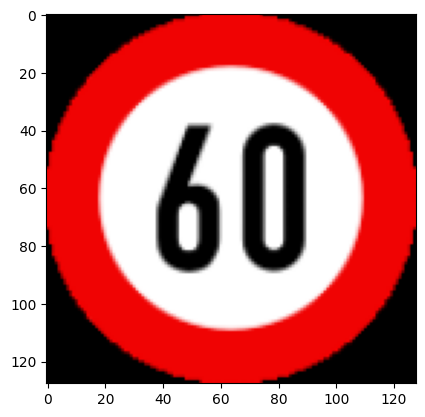
\includegraphics[width=0.3\textwidth]{color_histogram.png}
    \caption{Hình ảnh biển báo.}
    \vspace{0.5cm}
    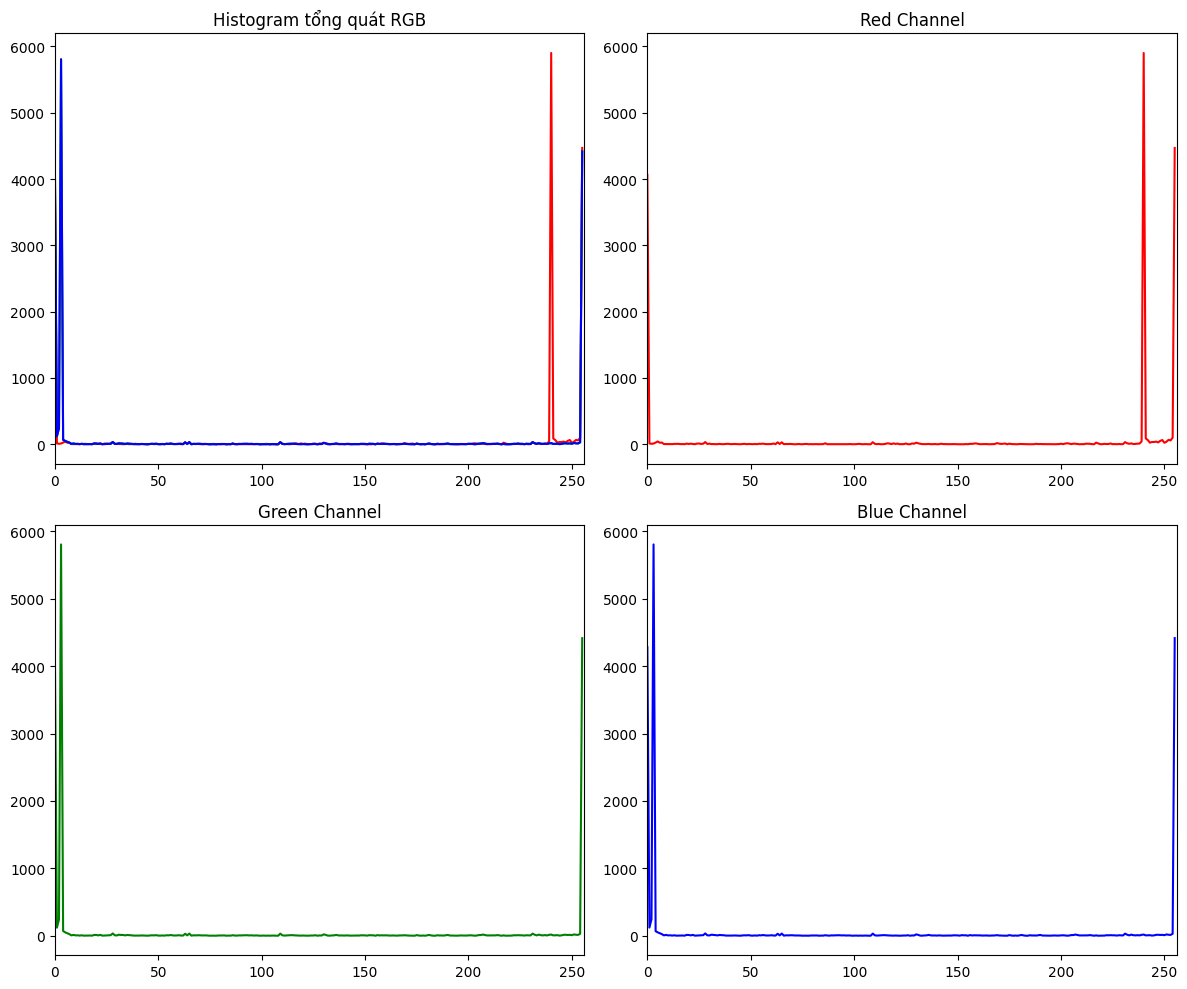
\includegraphics[width=0.9\textwidth]{color_histogram_extracted.png}
    \caption{Color Histogram được trích xuất từ hình ảnh biển báo (Hình 1).}
    \label{fig:color_histogram}
\end{figure}

\paragraph{Nhận xét về Color Histogram}
% \addcontentsline{toc}{subsubsection}{Nhận xét về Color Histogram}

\subparagraph{Ưu điểm}
- Đơn giản, dễ thực hiện và dễ dàng tích hợp vào hệ thống phân loại.\\
- Không phụ thuộc vào kích thước ảnh: Vì histogram chỉ phụ thuộc vào tần suất màu sắc, không bị ảnh hưởng bởi kích thước và tỷ lệ của ảnh.\\

\subparagraph{Nhược điểm}
- Không có thông tin về cấu trúc không gian: không phản ánh mối quan hệ không gian giữa các điểm ảnh, có thể ảnh hưởng đến hiệu suất trong một số bài toán phân loại phức tạp.\\

\subsubsection{Đặc trưng HOG}
% \addcontentsline{toc}{subsubsection}{Đặc trưng HOG}

\paragraph{Định nghĩa}
\hspace{5mm}HOG (Histogram of Oriented Gradients) là một phương pháp trích xuất đặc trưng từ ảnh dựa trên phân tích gradient. Các đặc trưng được xây dựng từ hướng gradient và magnitude của các pixel trong ảnh, sau đó phân nhóm chúng vào các bins (thùng chứa) để tạo thành một histogram. Phương pháp này chủ yếu được sử dụng trong các bài toán nhận dạng đối tượng và phát hiện biên của các đối tượng trong ảnh.

\paragraph{Nguyên lý hoạt động}
\hspace{5mm}HOG hoạt động bằng cách tính toán gradient của cường độ ánh sáng để xác định các cạnh và biên của đối tượng trong ảnh . Quá trình này bao gồm các bước chính như sau \cite{hog_opencv}:

\subparagraph{Tính Gradient}
\hspace{5mm}Bước đầu tiên trong việc tính toán HOG là tính gradient của hình ảnh để xác định hướng và độ mạnh của sự thay đổi trong cường độ sáng giữa các pixel. Sử dụng bộ lọc Sobel để tính toán gradient theo hai hướng \(x\) và \(y\), từ đó tính toán magnitude và direction của gradient từ các gradient \(x\) và \(y\).

\[
G = \sqrt{(G_x^2 + G_y^2)} \quad \text{\cite{hog_opencv}}
\]
\[
\theta = \arctan{\left(\frac{G_y}{G_x}\right)} \quad \text{\cite{hog_opencv}}
\]


\hspace{5mm}Trong đó:
\begin{itemize}
    \item \(G_x\) và \(G_y\) là gradient theo phương \(x\) và \(y\).
    \item \(G\) là magnitude của gradient.
    \item \(\theta\) là hướng gradient.
\end{itemize}

\subparagraph{Tạo ô (cell) và khối (block)}
\hspace{5mm}Sau khi tính gradient, ảnh được chia thành các ô nhỏ (cell) để tính toán histogram hướng trong mỗi ô. Mỗi ô có kích thước thường là \(8 \times 8\) pixel. Các ô này sau đó được nhóm thành các khối (block), mỗi block gồm 2x2 ô, tức là tổng cộng 16x16 pixel.

\subparagraph{Tạo histogram hướng trong mỗi ô}
\hspace{5mm}Mỗi ô sẽ tạo ra một histogram của các hướng gradient, trong đó hướng gradient được chia thành các bin. Thông thường, số bin là 9, với mỗi bin đại diện cho một khoảng góc từ 0 đến 180 độ, mỗi bin chiếm một khoảng góc 20 độ. Histogram này mô tả phân phối hướng gradient trong từng ô.

\subparagraph{Chuẩn hóa khối}
\hspace{5mm}Để giảm thiểu ảnh hưởng của sự thay đổi ánh sáng và độ tương phản, histogram của các ô trong mỗi khối sẽ được chuẩn hóa. Phương pháp chuẩn hóa phổ biến là L2-norm:

\[
\mathbf{v} = \frac{\mathbf{v}}{\sqrt{\|\mathbf{v}\|_2^2 + \epsilon^2}} \quad \text{\cite{hog_l2_norm}}
\]

Trong đó:
\begin{itemize}
    \item \(\mathbf{v}\) là vector đặc trưng của khối.
    \item \(\|\mathbf{v}\|_2\) là chuẩn L2 của vector \(\mathbf{v}\).
    \item \(\epsilon\) là một giá trị nhỏ (thường là \(10^{-6}\)) giúp tránh chia cho 0.
\end{itemize}

\subparagraph{Kết hợp đặc trưng}
\hspace{5mm}Cuối cùng, vector đặc trưng HOG được tạo ra bằng cách kết hợp các histogram chuẩn hóa từ tất cả các khối trong ảnh. Đây chính là đặc trưng HOG được sử dụng cho các tác vụ nhận dạng đối tượng.

\paragraph{Cài đặt trong bài toán}
\hspace{5mm}Đoạn mã Python dưới đây minh họa cách cài đặt HOG bằng thư viện `skimage`:

\begin{minted}[frame=single,fontsize=\footnotesize,linenos]{python}
from skimage.feature import hog

def hog_features(image):
    hog_features = hog(image, orientations=9, pixels_per_cell=(8, 8), 
                       cells_per_block=(2, 2), visualize=False, 
                       block_norm='L2-Hys', transform_sqrt=True, 
                       channel_axis=2)
    return hog_features
\end{minted}

\noindent Giải thích các tham số trong hàm \texttt{hog}:
\begin{itemize}
    \item \texttt{image}: Ảnh đầu vào, có thể là ảnh màu (RGB) hoặc ảnh xám (grayscale).
    \item \texttt{orientations}: Số lượng bins trong histogram hướng gradient. Trong ví dụ này, giá trị là 9, có nghĩa là các hướng gradient sẽ được phân chia thành 9 bins, mỗi bin đại diện cho một phạm vi góc từ 0 đến 180 độ.
    \item \texttt{pixels\_per\_cell}: Kích thước của mỗi ô (cell) trong ảnh, được xác định là \(8 \times 8\) pixel. Mỗi cell sẽ tính toán gradient và độ mạnh (magnitude) của pixel trong đó.
    \item \texttt{cells\_per\_block}: Số lượng ô (cell) trong một block, được xác định là 2x2 ô, tức là mỗi block có kích thước \(16 \times 16\) pixel.
    \item \texttt{visualize}: Điều khiển việc có hay không trực quan hóa các đặc trưng HOG dưới dạng ảnh. Nếu \texttt{True}, hàm sẽ trả về cả ảnh biểu diễn các đặc trưng HOG.
    \item \texttt{block\_norm}: Phương pháp chuẩn hóa trong mỗi block. "L2-Hys" là một phương pháp chuẩn hóa phổ biến trong HOG, giúp giảm ảnh hưởng của ánh sáng và độ tương phản. Phương pháp chuẩn hóa L2-Hys \cite{hog_l2_norm} có thể được mô tả bằng các bước sau:

    \[
    \mathbf{v'} = \frac{\mathbf{v}}{\sqrt{\|\mathbf{v}\|_2^2 + \epsilon^2}} \quad \text{(bước 1: chuẩn hóa L2)}
    \]

    Sau đó, giá trị của vector \(\mathbf{v'}\) sẽ bị cắt (clip) nếu vượt quá ngưỡng \(0.2\):

    \[
    \mathbf{v'} = \min(\mathbf{v'}, 0.2) \quad \text{(bước 2: cắt giá trị)}
    \]

    Cuối cùng, chuẩn hóa lại vector sau khi cắt:

    \[
    \mathbf{v'} = \frac{\mathbf{v'}}{\sqrt{\|\mathbf{v'}\|_2^2 + \epsilon^2}} \quad \text{(bước 3: chuẩn hóa L2 lại sau khi cắt)}
    \]

    Trong đó:
    \begin{itemize}
        \item \(\mathbf{v}\) là vector đặc trưng của block.
        \item \(\|\mathbf{v}\|_2\) là chuẩn L2 của vector \(\mathbf{v}\).
        \item \(\epsilon\) là một hằng số nhỏ (thường là \(10^{-6}\)) để tránh chia cho 0.
        \item \(\mathbf{v'}\) là vector đã được chuẩn hóa và cắt.
    \end{itemize}
    Phương pháp chuẩn hóa L2-Hys giúp giảm ảnh hưởng của sự thay đổi độ sáng và độ tương phản đồng thời làm ổn định quá trình huấn luyện mô hình.
    
    \item \texttt{transform\_sqrt}: Áp dụng phép biến đổi căn bậc 2 vào các giá trị độ sáng trong ảnh trước khi tính gradient. Điều này giúp giảm bớt sự ảnh hưởng của sự khác biệt lớn về độ sáng giữa các phần khác nhau của ảnh.
    \item \texttt{channel\_axis}: Tham số này chỉ định kênh màu của ảnh. Nếu ảnh là ảnh màu, tham số này giúp hàm phân tích các kênh màu riêng biệt (Red, Green, Blue).
\end{itemize}

\noindent
\textbf{Hình minh họa:}
\begin{figure}[H]
    \centering
    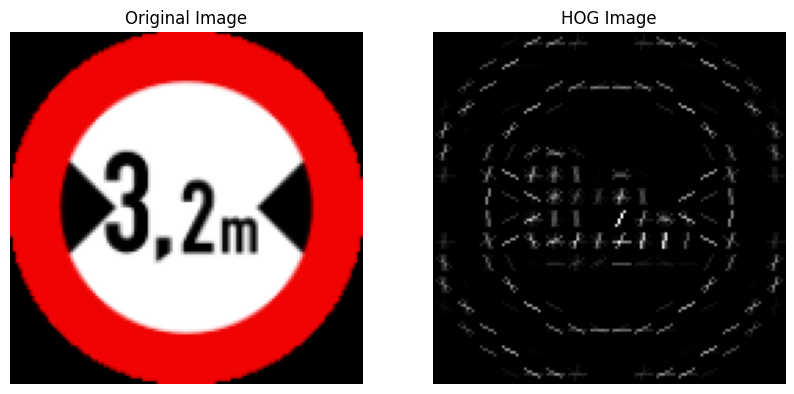
\includegraphics[width=0.7\textwidth]{original_and_hog_extracted.png}
    \caption{\centering (Trái) Hình ảnh biển báo và (Phải) Đặc trưng HOG được trích xuất từ ảnh biển báo.}
    \label{fig:hog}
\end{figure}

\paragraph{Nhận xét về HOG}

\subparagraph{Ưu điểm}
\begin{itemize}
    \item \textbf{Tính hiệu quả cao trong nhận dạng đối tượng:} HOG rất phù hợp trong các bài toán phát hiện đối tượng, đặc biệt là trong nhận dạng khuôn mặt và các đối tượng có biên rõ ràng.
    \item \textbf{Khả năng chống lại sự thay đổi độ sáng và độ tương phản:} Phương pháp chuẩn hóa L2 giúp giảm thiểu sự ảnh hưởng của các thay đổi ánh sáng và độ tương phản, làm tăng khả năng nhận diện đối tượng trong môi trường khác nhau.
\end{itemize}

\subparagraph{Nhược điểm}
\begin{itemize}
    \item \textbf{Tính toán phức tạp:} Quá trình tính toán gradient và chuẩn hóa có thể tốn nhiều tài nguyên tính toán, đặc biệt là với các ảnh có độ phân giải cao.
    \item \textbf{Không hiệu quả với các đối tượng có biên mờ hoặc có kết cấu phức tạp:} HOG chủ yếu hoạt động tốt với các đối tượng có biên rõ ràng, trong khi các đối tượng mờ hoặc không rõ ràng có thể làm giảm hiệu quả của phương pháp này.
\end{itemize}
\vspace{5mm}


\subsubsection{Tổng hợp đặc trưng}
\label{subsubsec:tong-hop-dac-trung}

\begin{minted}[frame=single,fontsize=\footnotesize,linenos]{python}
def blur_image(image):
    gaussian_blurred_image = cv2.GaussianBlur(image, (5, 5), 0)
    # blurred_image = cv2.medianBlur(image, 5)
    return blurred_image

def extract_features(images):
    blurred_images = [blur_image(image) for image in images]
    color_features = [color_histogram(image) for image in blurred_images]
    hog_features = [hog(image) for image in blurred_images]
    combined_features = [np.concatenate((color_feature, hog_feature)) 
                        for color_feature, hog_feature 
                        in zip(color_features, hog_features)]
    return combined_features
\end{minted}

\noindent Giải thích code:

\begin{itemize}
    \item \texttt{blur\_image}: Hàm này áp dụng phương pháp làm mờ lên ảnh đầu vào. Có hai phương pháp làm mờ được sử dụng trong đó:
    
    \begin{itemize}
        \item \texttt{GaussianBlur}: Phương pháp này áp dụng bộ lọc Gaussian để làm mờ ảnh. Bộ lọc Gaussian sử dụng hàm Gaussian để tính toán trọng số cho mỗi pixel trong ảnh, giúp làm mịn các chi tiết ảnh. Công thức Gaussian là:
        
        \[
        G(x, y) = \frac{1}{2\pi\sigma^2} e^{-\frac{x^2 + y^2}{2\sigma^2}}
        \quad \text{\cite{nixonaguado_gaussianblur}}
        \]
        Trong đó:
        \begin{itemize}
            \item \(x, y\) là tọa độ pixel trong không gian ảnh.
            \item \(\sigma\) là độ lệch chuẩn, điều chỉnh độ rộng của bộ lọc (càng lớn \(\sigma\), ảnh càng mờ).
        \end{itemize}
        
        \item \texttt{medianBlur}: Đây là phương pháp làm mờ sử dụng bộ lọc trung vị, trong đó mỗi pixel trong ảnh được thay thế bằng giá trị trung vị của một vùng lân cận. Công thức cho median blur là:
        
        \[
        I'(x, y) = \text{median}\left(I(x', y') \mid (x', y') \in \text{kernel}\right)
        \quad \text{\cite{nixonaguado_medianblur}}
        \]
        Trong đó:
        \begin{itemize}
            \item \(I(x, y)\) là giá trị pixel tại vị trí \((x, y)\).
            \item \(\text{kernel}\) là vùng lân cận (có thể có kích thước 3x3, 5x5, v.v.) quanh pixel \((x, y)\).
        \end{itemize}
    \end{itemize}
    
    \noindent So sánh giữa \texttt{GaussianBlur} và \texttt{medianBlur}:
    \begin{itemize}
        \item \textbf{Gaussian Blur}: Là phép làm mờ ảnh dựa trên trọng số, trong đó mỗi pixel trong ảnh được thay thế bằng giá trị trung bình có trọng số của các pixel xung quanh, với trọng số tuân theo phân phối Gaussian. Phương pháp này giúp làm mờ các chi tiết nhỏ và giảm nhiễu, nhưng có thể làm mờ các biên ảnh (edges) và mất chi tiết quan trọng. Nhiễu dạng Gaussian thường xuất hiện khi tín hiệu ảnh bị nhiễu do các yếu tố ngẫu nhiên như cảm biến máy ảnh hoặc môi trường ánh sáng không ổn định, và nó có phân bố chuẩn.
        
        \item \textbf{Median Blur}: Là phép làm mờ ảnh bằng cách thay thế mỗi pixel trong ảnh bằng giá trị trung vị của vùng lân cận. Phương pháp này rất hiệu quả trong việc loại bỏ các nhiễu xuất hiện đột ngột và không có quy luật, nhưng không làm mờ các chi tiết ảnh mạnh như Gaussian Blur. Median Blur giữ được biên ảnh rõ ràng hơn và không làm mất chi tiết quá nhiều. Tuy nhiên, nó không hiệu quả trong việc giảm nhiễu dạng Gaussian vì không sử dụng trọng số và chỉ dựa vào giá trị trung vị. (Nhiễu dạng Gaussian là dạng nhiễu có phân bố chuẩn (Gaussian distribution), thường gặp trong các tín hiệu ảnh bị nhiễu do các yếu tố ngẫu nhiên như ánh sáng không ổn định hoặc cảm biến máy ảnh. Nó ảnh hưởng đến tất cả các pixel trong ảnh theo phân bố chuẩn.)
    \end{itemize}
    
    \item \texttt{blurred\_images}: Là một danh sách chứa các ảnh đã được làm mờ bằng phương pháp \texttt{blur\_image}.
    
    \item \texttt{color\_features}: Là một danh sách chứa các đặc trưng màu sắc của các ảnh đã được làm mờ. Hàm \texttt{color\_histogram} tính toán histogram màu cho mỗi ảnh. Đây là một cách phổ biến để trích xuất đặc trưng màu sắc từ ảnh.
    
    \item \texttt{hog\_features}: Là một danh sách chứa các đặc trưng HOG (Histogram of Oriented Gradients) của các ảnh đã được làm mờ. Hàm \texttt{hog} tính toán các đặc trưng hướng gradient của mỗi ảnh. HOG là một phương pháp đặc trưng mạnh mẽ để nhận dạng đối tượng, đặc biệt trong các tác vụ nhận dạng hình ảnh.
    
    \item \texttt{combined\_features}: Là một danh sách chứa các đặc trưng kết hợp giữa \texttt{color\_features} và \texttt{hog\_features}. Hàm \texttt{np.concatenate} được sử dụng để ghép nối các đặc trưng màu sắc và HOG thành một vector đặc trưng duy nhất cho mỗi ảnh.
\end{itemize}

\noindent Cuối cùng, hàm \texttt{extract\_features} trả về danh sách các đặc trưng kết hợp cho tất cả các ảnh đầu vào.

\subsection{Thuật toán máy học}

\subsubsection{Thuật toán K-Nearest Neighbors (KNN)}

\paragraph{Nguồn gốc}
\begin{itemize}
    \item \textbf{1951 - Evelyn Fix \& Joseph Hodges:} Đưa ra khái niệm K-nearest neighbors (KNN) như một phương pháp phân loại không tham số, không giả định về phân phối dữ liệu \cite{fix_hodges_1951, fix1951}.
    \item \textbf{1967 - Thomas Cover \& Peter Hart:} Mở rộng và phát triển thuật toán KNN, chứng minh tính nhất quán trong lý thuyết quyết định \cite{cover1967}.
\end{itemize}
\textbf{Tính Nhất Quán (Consistency):} Khi số lượng dữ liệu huấn luyện tăng lên vô hạn, thuật toán KNN sẽ hội tụ và đạt được hiệu suất tối ưu tương tự như phương pháp phân loại lý tưởng (tức là phương pháp có tỷ lệ lỗi thấp nhất có thể).

\paragraph{Nguyên lý hoạt động}
\hspace{5mm}Thuật toán K-Nearest Neighbors (KNN) bao gồm ba bước chính \cite{knnprinciple} như sau:

\subparagraph{Tính khoảng cách}  
\hspace{5mm}KNN tính toán khoảng cách giữa điểm cần dự đoán và tất cả các điểm trong tập huấn luyện. Một số loại khoảng cách phổ biến bao gồm:
\begin{itemize}
    \item \textbf{Euclidean Distance:}
    \[
    d(p, q) = \sqrt{\sum_{i=1}^{n} (p_i - q_i)^2}
    \]
    Khoảng cách này đo độ dài đoạn thẳng nối hai điểm \(p\) và \(q\).
    
    \item \textbf{Manhattan (Cityblock) Distance:}
    \[
    d(p, q) = \sum_{i=1}^{n} |p_i - q_i|
    \]
    Được tính bằng tổng độ dài các đoạn song song với các trục tọa độ.

    \item \textbf{Cosine Similarity (Ngược lại là Cosine Distance):}
    \[
    \text{cosine\_distance}(p, q) = 1 - \frac{\sum_{i=1}^n p_i q_i}{\sqrt{\sum_{i=1}^n p_i^2} \sqrt{\sum_{i=1}^n q_i^2}}
    \]
    Đo lường độ tương đồng giữa hai vector, thường được sử dụng trong các bài toán phân tích văn bản hoặc dữ liệu nhiều chiều.

    \item \textbf{Squared Euclidean Distance:}
    \[
    d(p, q) = \sum_{i=1}^{n} (p_i - q_i)^2
    \]
    Đây là bình phương của khoảng cách Euclidean, thường được dùng để giảm chi phí tính căn bậc hai.

    \item \textbf{Chi-Square Distance:}
    \[
    d(p, q) = \sum_{i=1}^{n} \frac{(p_i - q_i)^2}{p_i + q_i}
    \]
    Sử dụng phổ biến trong bài toán xử lý dữ liệu histogram.

    \item \textbf{Bhattacharyya Distance:}
    \[
    d(p, q) = -\ln \left(\sum_{i=1}^{n} \sqrt{p_i q_i}\right)
    \]
    Được dùng để đo độ tương đồng giữa hai phân phối xác suất.

    \item \textbf{Intersection Distance:}
    \[
    d(p, q) = \sum_{i=1}^{n} \min(p_i, q_i)
    \]
    Hiệu quả khi làm việc với các giá trị không âm, ví dụ như histogram.
\end{itemize}

\subparagraph{Tìm \(K\) điểm gần nhất}  
\hspace{5mm}Sau khi tính toán khoảng cách, thuật toán chọn \(K\) điểm dữ liệu có khoảng cách ngắn nhất tới điểm dữ liệu cần dự đoán. \(K\) là một tham số được chọn trước, ảnh hưởng đến hiệu suất của thuật toán. Nếu \(K\) quá nhỏ, mô hình có thể dễ bị nhiễu. Nếu \(K\) quá lớn, mô hình có thể mất đi độ chính xác do ảnh hưởng của các điểm không liên quan.

\subparagraph{Dự đoán nhãn}  
\hspace{5mm}KNN dự đoán nhãn của điểm mới dựa trên các nhãn của \(K\) điểm gần nhất. Các phương pháp dự đoán nhãn bao gồm:
\begin{itemize}
    \item \textbf{Biểu quyết đa số (Majority Voting):} Nhãn được xác định bằng nhãn xuất hiện nhiều nhất trong \(K\) điểm gần nhất. Công thức:
    \[
    \hat{y} = \arg \max_y \sum_{i=1}^K \mathbb{I}(y_i = y)
    \]
    Trong đó:
    \begin{itemize}
        \item \(\mathbb{I}(y_i = y)\) là hàm chỉ thị, nhận giá trị 1 nếu \(y_i = y\), và 0 trong trường hợp ngược lại.
    \end{itemize}

    \item \textbf{Trọng số theo khoảng cách (Distance-Weighted Voting):} Mỗi láng giềng được gán một trọng số tỷ lệ nghịch với khoảng cách. Công thức:
    \[
    \hat{y} = \arg \max_y \sum_{i=1}^K \frac{\mathbb{I}(y_i = y)}{d(p, q_i) + \epsilon}
    \]
    Trong đó:
    \begin{itemize}
        \item \(d(p, q_i)\) là khoảng cách từ điểm cần dự đoán \(p\) tới láng giềng \(q_i\).
        \item \(\epsilon\) là một giá trị rất nhỏ để tránh chia cho 0.
    \end{itemize}
\end{itemize}

\paragraph{Cài đặt thuật toán}

\begin{minted}[frame=single,fontsize=\footnotesize,linenos]{python}
from sklearn.neighbors import KNeighborsClassifier

knn_model = KNeighborsClassifier(
    n_neighbors=5, 
    weights='distance', 
    metric='euclidean'
)
knn_model.fit(X_train, y_train)
y_pred = knn_model.predict(X_test)
\end{minted}

\noindent \textbf{Giải thích các tham số}
\begin{itemize}
    \item \texttt{n\_neighbors}: Số lượng láng giềng gần nhất được sử dụng để xác định nhãn của một điểm mới.
    \begin{itemize}
        \item Giá trị này ảnh hưởng trực tiếp đến độ chính xác và độ nhạy của mô hình.
        \item Với \texttt{n\_neighbors=5}, nhãn của điểm mới được xác định bởi 5 láng giềng gần nhất trong không gian đặc trưng.
    \end{itemize}

    \item \texttt{weights}: Quy định cách tính trọng số của các láng giềng khi dự đoán nhãn.
    \begin{itemize}
        \item \texttt{'uniform'}: Mọi láng giềng có trọng số như nhau.
        \item \texttt{'distance'}: Láng giềng gần hơn có trọng số lớn hơn (dựa trên khoảng cách).
    \end{itemize}
    
    \item \texttt{metric}: Định nghĩa loại khoảng cách được sử dụng để tính toán láng giềng. Các công thức metric đã được giải thích ở phần \textbf{Nguyên lý hoạt động}.
\end{itemize}

\subsubsection{Thuật toán Support Vector Machine (SVM)}

\paragraph{Nguồn gốc}
\begin{itemize}
    \item \textbf{1974 - Vladimir Vapnik và Alexey Chervonenkis:} Phát triển lý thuyết VC (Vapnik–Chervonenkis), đặt nền tảng lý thuyết cho các thuật toán học máy dựa trên biên tối đa và khả năng tổng quát hóa, cơ sở cho việc xây dựng SVM \cite{vapnik1974}.
    \item \textbf{1982, 1995 - Vladimir Vapnik:} Giới thiệu thuật toán SVM, tập trung vào mô hình phân loại tuyến tính dựa trên nguyên lý biên tối đa. SVM sử dụng siêu phẳng tối ưu để phân chia các lớp dữ liệu, giảm thiểu lỗi phân loại \cite{vapnik1995}.
    \item \textbf{1992 - Bernhard Boser, Isabelle Guyon và Vladimir Vapnik:} Đề xuất kernel trick, mở rộng khả năng của SVM để giải quyết các bài toán phân loại phi tuyến \cite{boser1992}.
\end{itemize}

\paragraph{Nguyên lý hoạt động}
\hspace{5mm}SVM tìm kiếm một siêu phẳng (hyperplane) tối ưu trong không gian đặc trưng để phân chia các lớp dữ liệu sao cho khoảng cách giữa siêu phẳng và các điểm dữ liệu gần nhất (support vectors) là lớn nhất. Mục tiêu là tối đa hóa biên (margin), tức là khoảng cách giữa siêu phẳng và các điểm dữ liệu của các lớp khác nhau.

\subparagraph{Tìm siêu phẳng tối ưu}  
\hspace{5mm}Mục tiêu của SVM là tìm một siêu phẳng tối ưu trong không gian đặc trưng sao cho khoảng cách giữa siêu phẳng và các điểm gần nhất từ mỗi lớp (support vectors) là lớn nhất. Điều này tương đương với việc tối đa hóa biên (margin), được tính bởi:

\[
\text{Margin} = \frac{2}{\|\mathbf{w}\|} \quad \text{\cite{svm_margin}}
\]
Trong đó:
\begin{itemize}
    \item \(\mathbf{w}\) là vector trọng số của siêu phẳng.
\end{itemize}

\subparagraph{Hàm mục tiêu trong SVM}  
\hspace{5mm}Hàm mục tiêu của SVM là tối thiểu hóa hàm chi phí, bao gồm hai thành phần: một phần về sai số (penalty) và một phần về biên tối đa. Công thức hàm mục tiêu là:

\[
\min_{\mathbf{w}, b} \frac{1}{2} \|\mathbf{w}\|^2 \quad \text{với điều kiện} \quad y_i (\mathbf{w} \cdot \mathbf{x}_i + b) \geq 1 \quad \forall i
\quad \text{\cite{boser1992}}
\]
Trong đó:
\begin{itemize}
    \item \(\mathbf{w}\) là vector trọng số.
    \item \(b\) là bias (hệ số bù).
    \item \(y_i\) là nhãn của điểm dữ liệu (\(y_i = \pm 1\)).
    \item \(\mathbf{x}_i\) là điểm dữ liệu.
\end{itemize}
\hspace{5mm}Năm 1995, Corinna Cortes và Vladimir N. Vapnik đề xuất một ý tưởng mới cho phép thuật toán gán nhãn sai cho một số mẫu luyện tập. Nếu không tồn tại siêu phẳng nào phân tách được hai lớp dữ liệu, thì thuật toán \textbf{Biên mềm} sẽ chọn một siêu phẳng phân tách các mẫu luyện tập tốt nhất có thể, và đồng thời cực đại hóa khoảng cách giữa siêu phẳng với các mẫu được gán đúng nhãn. Phương pháp này sử dụng các biến bù $\xi_i$ dùng để đo độ sai lệch của mẫu $x_i$. Hàm mục tiêu có thêm một số hạng mới để phạt thuật toán khi $\xi_i$ khác không, và bài toán tối ưu hóa trở thành việc trao đổi giữa độ lứa của biên và mức phạt nhỏ. Theo đó hàm mục tiêu trở thành:
\[
\min_{\mathbf{w}, b,\xi_i} \frac{1}{2} \|\mathbf{w}\|^2 \quad  + C\sum^i{}\text{với điều kiện} \quad y_i (\mathbf{w} \cdot \mathbf{x}_i + b) \geq 1 \quad \forall i
\quad \text{\cite{svm_wiki}}
\]

\subparagraph{Kernel Trick (Nếu dữ liệu phi tuyến)}  
\hspace{5mm}Nếu dữ liệu không thể phân chia một cách rõ ràng bằng siêu phẳng trong không gian gốc (dữ liệu phi tuyến), SVM sử dụng kernel trick để ánh xạ dữ liệu vào không gian đặc trưng cao hơn, nơi phân chia trở thành tuyến tính. Hàm kernel \(K(\mathbf{x}_i, \mathbf{x}_j)\) có thể tính toán khoảng cách trong không gian cao mà không cần tính toán trực tiếp các tọa độ trong không gian đó. Một số hàm kernel phổ biến \cite{svm_kernel}

\begin{itemize}
    \item \textbf{Linear kernel:}
    \[
    K(\mathbf{x}_i, \mathbf{x}_j) = \mathbf{x}_i^T \mathbf{x}_j
    \]
    \begin{itemize}
        \item Kernel tuyến tính đơn giản, sử dụng tích vô hướng giữa hai điểm dữ liệu.
    \end{itemize}
    \item \textbf{Polynomial kernel:}
    \[
    K(\mathbf{x}_i, \mathbf{x}_j) = (\mathbf{x}_i^T \mathbf{x}_j + 1)^d
    \]
    \begin{itemize}
        \item Với \(d\) là bậc của đa thức, giúp mô hình học các biên phân tách phi tuyến phức tạp.
    \end{itemize}
    \item \textbf{Radial Basis Function (RBF) kernel:}
    \[
    K(\mathbf{x}_i, \mathbf{x}_j) = \exp\left(-\frac{\|\mathbf{x}_i - \mathbf{x}_j\|^2}{2\sigma^2}\right)
    \]
    \begin{itemize}
        \item Kernel Gaussian, sử dụng khoảng cách Euclid để tính toán ảnh hưởng của các điểm dữ liệu.
    \end{itemize}
    \item \textbf{Sigmoid kernel:}
    \[
    K(\mathbf{x}_i, \mathbf{x}_j) = \tanh\left(\alpha \mathbf{x}_i^T \mathbf{x}_j + c\right)
    \]
    \begin{itemize}
        \item Kernel sigmoid mô phỏng hàm kích hoạt trong mạng nơ-ron.
        \item Tham số \(\alpha\) điều chỉnh độ dốc, và \(c\) là hằng số dịch chuyển.
    \end{itemize}
\end{itemize}


\subparagraph{Dự đoán nhãn}  
\hspace{5mm}Sau khi tìm được siêu phẳng tối ưu, SVM sử dụng siêu phẳng này để phân loại điểm mới. Điểm mới sẽ được phân vào lớp bên kia của siêu phẳng, tùy thuộc vào phía của siêu phẳng mà nó nằm. Hàm phân loại là:

\[
\hat{y} = \text{sign}(z), \quad \text{với} \; z = \mathbf{w} \cdot \mathbf{x} + b
\]

\noindent Trong đó:
\begin{itemize}
    \item \(z\) là giá trị kết hợp tuyến tính của vector trọng số, vector đặc trưng và bias.
    \item \(\mathbf{w}\) là vector trọng số.
    \item \(\mathbf{x}\) là vector đặc trưng của điểm cần phân loại.
    \item \(b\) là bias.
    \item \(\text{sign}(z)\) trả về \(+1\) nếu \(z \geq 0\) và \(-1\) nếu \(z < 0\).
\end{itemize}


\paragraph{Cài đặt thuật toán}

\begin{minted}[frame=single,fontsize=\footnotesize,linenos]{python}
from sklearn.svm import SVC

svc_model = SVC(C=1.0, degree=3, gamma=0.1, kernel='poly')
svc_model.fit(X_train, y_train)
y_pred = svc_model.predict(X_test)
\end{minted}

\noindent \textbf{Giải thích các tham số}
\begin{itemize}
    \item \texttt{C}: Tham số điều chỉnh mức phạt đối với các lỗi phân loại.
    \begin{itemize}
        \item Giá trị nhỏ (ví dụ: C=0.1): Mô hình cho phép một số lỗi khi phân loại, điều này giúp mô hình dễ dàng chấp nhận sự không hoàn hảo trong dữ liệu và có khả năng tổng quát tốt hơn khi áp dụng vào dữ liệu mới.
        \item Giá trị lớn (ví dụ: C=10): Mô hình yêu cầu phân loại chính xác hơn, ít chấp nhận lỗi, nhưng dễ dẫn đến overfitting.
    \end{itemize}

    \item \texttt{degree}: Bậc của đa thức trong kernel='poly'. Quyết định độ phức tạp của mô hình khi sử dụng kernel đa thức.
    \begin{itemize}
        \item Với \texttt{degree=3}, hàm kernel sẽ tương ứng với một đa thức bậc ba, giúp mô hình có khả năng học các đường biên phi tuyến phức tạp hơn.
    \end{itemize}

    \item \texttt{gamma}: Hệ số quyết định mức độ ảnh hưởng của một điểm dữ liệu đơn lẻ trong hàm kernel.
    \begin{itemize}
        \item Giá trị nhỏ (ví dụ: gamma=0.1) làm tăng mức độ ảnh hưởng, dẫn đến một mô hình tổng quát hóa tốt hơn nhưng ít chi tiết hơn.
        \item Giá trị lớn (ví dụ: gamma=10) làm giảm mức độ ảnh hưởng, mô hình tập trung hơn vào các điểm dữ liệu gần, dễ overfit.
    \end{itemize}

    \item \texttt{kernel}: Hàm kernel được sử dụng để ánh xạ dữ liệu từ không gian gốc sang không gian đặc trưng cao hơn.
    \begin{itemize}
        \item \texttt{'poly'}: Sử dụng kernel đa thức, phù hợp cho các bài toán với biên phi tuyến phức tạp có thể được biểu diễn bằng đa thức.
        \item \texttt{'linear'}: Sử dụng kernel tuyến tính.
        \item \texttt{'rbf'}: Kernel Gaussian, phù hợp cho các biên phân tách phi tuyến mượt.
        \item \texttt{'sigmoid'}: Kernel sigmoid, mô phỏng hàm kích hoạt của mạng nơ-ron.
    \end{itemize}
\end{itemize}

\subsection{Phương pháp GridSearchCV}

\hspace{5mm}GridSearchCV là một kỹ thuật quan trọng trong học máy, được sử dụng để tối ưu hóa tham số siêu (\textit{hyperparameters}) nhằm tìm ra các giá trị tốt nhất cho một mô hình. Hiệu suất của một mô hình học máy phụ thuộc rất lớn vào các tham số siêu, vì chúng kiểm soát cách thức mô hình học và đưa ra quyết định. Tuy nhiên, việc xác định giá trị tối ưu cho các tham số siêu thường không thể biết trước và đòi hỏi quá trình thử nghiệm.

\subsubsection{Nguyên lý hoạt động} 
\hspace{5mm}GridSearchCV tự động hóa quá trình thử nghiệm các giá trị tham số siêu bằng cách thực hiện kiểm tra toàn diện trên tất cả các tổ hợp giá trị được xác định trước trong một không gian tham số. Sau khi thử nghiệm, GridSearchCV sẽ chọn ra tổ hợp tham số mang lại hiệu suất tốt nhất dựa trên một tiêu chí đánh giá nhất định, chẳng hạn như \textit{accuracy}, \textit{precision}, \textit{recall}, hay \textit{f1-score}.

\subsubsection{Nhận xét chung về GridsearchCV}

\paragraph{Ưu điểm}
\hspace{5mm}Việc thử nghiệm thủ công tất cả các tổ hợp tham số có thể rất tốn thời gian và công sức, đặc biệt đối với các mô hình phức tạp và tập dữ liệu lớn. GridSearchCV giúp tự động hóa quy trình này, tiết kiệm thời gian hơn so với phương pháp thủ công, đồng thời đảm bảo rằng mọi tổ hợp tham số đều được xem xét một cách hệ thống.

\paragraph{Nhược điểm}
\hspace{5mm}Quá trình thử nghiệm có thể rất tốn kém về mặt thời gian khi số lượng tham số và giá trị của chúng là rất lớn. Với các mô hình phức tạp, GridSearchCV có thể phải thử nghiệm một số lượng tổ hợp tham số cực kỳ lớn, điều này làm tăng thời gian huấn luyện. Hơn nữa, GridSearchCV không tối ưu hoá được việc lựa chọn tham số trong một không gian rộng lớn và có thể bỏ sót các kết quả tốt hơn nếu không gian tham số không được định nghĩa hợp lý.

\subsubsection{Ứng dụng} 
\hspace{5mm}GridSearchCV được tích hợp trong thư viện \texttt{scikit-learn}, thuộc gói \newline \texttt{model\_selection}. Nó hỗ trợ nhiều kỹ thuật đo lường hiệu suất để đảm bảo rằng mô hình không chỉ đạt hiệu suất cao trên tập huấn luyện mà còn hoạt động tốt trên dữ liệu chưa nhìn thấy, giúp giảm thiểu hiện tượng quá khớp (\textit{overfitting}).\\

\noindent Cú pháp cơ bản của GridSearchCV thường bao gồm các thành phần chính \cite{gridsearchcv_mygreatlearning}:
\begin{itemize}
    \item \texttt{estimator}: Mô hình học máy cần tối ưu hóa, ví dụ \texttt{KNeighborsClassifier}, \texttt{SVC}, \texttt{RandomForestClassifier}, v.v. Đây là tham số bắt buộc phải có.
    \item \texttt{param\_grid}: Một từ điển hoặc danh sách các từ điển, chứa các tham số cần tối ưu và các giá trị tương ứng để thử nghiệm.
    %     \begin{minted}[frame=single,fontsize=\footnotesize,linenos]{python}
    %     param_grid = {
    %         'n_neighbors': [3, 5, 7],
    %         'weights': ['uniform', 'distance']
    %     }
    %     \end{minted}
    % GridSearchCV sẽ thử nghiệm tất cả các tổ hợp giá trị này.
    \item \texttt{cv}: Số lượng lần chia nhỏ dữ liệu để thực hiện \textit{cross-validation}. Khi \texttt{cv=k}, dữ liệu sẽ được chia thành \(k\) tập con. Trong mỗi lần thử nghiệm, một tập con được sử dụng để đánh giá và \(k-1\) tập con còn lại được dùng để huấn luyện. Điều này đảm bảo mô hình được đánh giá toàn diện và hiệu quả.
    \item \texttt{scoring}: Tiêu chí đánh giá hiệu suất của mô hình. GridSearchCV hỗ trợ nhiều độ đo khác nhau, như \texttt{'accuracy'}, \texttt{'f1\_macro'}, \texttt{'roc\_auc'}, v.v., tùy thuộc vào bài toán cụ thể. Người dùng có thể chọn tiêu chí phù hợp để tối ưu hóa mô hình.
    \item \texttt{verbose}: Mức độ chi tiết khi hiển thị kết quả trong quá trình tìm kiếm. Tham số này có thể nhận các giá trị từ 0 đến 3, với \texttt{verbose=0} là mức yên lặng hoàn toàn và \texttt{verbose=3} hiển thị thông tin chi tiết nhất.
\end{itemize}

\subsubsection{GridSearchCV cho KNN}  
\hspace{5mm}Trong bài toán này, GridSearchCV được áp dụng để tối ưu hóa các siêu tham số cho mô hình \(k\)-Nearest Neighbors (KNN). Các siêu tham số cần tối ưu hóa bao gồm:  
\begin{itemize}
    \item \texttt{n\_neighbors}: Số lượng hàng xóm gần nhất được xét để dự đoán.
    \item \texttt{weights}: Phương pháp tính trọng số khi lấy trung bình (\texttt{uniform} sử dụng trọng số đều, \texttt{distance} sử dụng trọng số ngược khoảng cách).
    \item \texttt{metric}: Hàm khoảng cách được sử dụng để đo độ tương đồng giữa các điểm, bao gồm:
    \begin{itemize}
        \item \texttt{cityblock}: Khoảng cách Manhattan.
        \item \texttt{cosine}: Khoảng cách Cosine.
        \item \texttt{sqeuclidean}: Khoảng cách Euclid bình phương.
        \item \texttt{chi\_square\_distance}: Khoảng cách \(\chi^2\).
        \item \texttt{bhattacharyya\_distance}: Khoảng cách Bhattacharyya.
        \item \texttt{intersection\_distance}: Khoảng cách giao nhau.
    \end{itemize}
\end{itemize}

Cài đặt GridSearchCV để tìm tham số tốt nhất cho mô hình KNN:

\begin{minted}[frame=single,fontsize=\footnotesize,linenos]{python}
from sklearn.neighbors import KNeighborsClassifier
from sklearn.model_selection import GridSearchCV

# Định nghĩa không gian tham số
param_grid = {
    'n_neighbors': [3, 4, 5, 6, 7, 10],
    'weights': ['uniform', 'distance'],
    'metric': [
        'cityblock', 'cosine',
        'sqeuclidean', 'chi_square_distance',
        'bhattacharyya_distance', 'intersection_distance'
    ]
}

# Khởi tạo mô hình k-NN
knn_model = KNeighborsClassifier()

# Grid Search
grid_search_knn = GridSearchCV(
    knn_model,
    param_grid,
    cv=3,
    scoring='f1_macro',
    verbose=3 
)

# Huấn luyện mô hình
grid_search_knn.fit(X_train, y_train)
\end{minted}

\noindent \textbf{Giải thích các tham số chính:}
\begin{itemize}
    \item \texttt{cv=3}: Số lượng lần chia nhỏ dữ liệu để thực hiện Cross-Validation. Khi \texttt{cv=3}, dữ liệu được chia thành 3 tập con (folds). Trong mỗi lần thử nghiệm, một tập được dùng để đánh giá và hai tập còn lại được sử dụng để huấn luyện. Điều này đảm bảo tính tổng quát và ổn định trong đánh giá mô hình.
    
    \item \texttt{scoring='f1\_macro'}: Đây là tiêu chí đánh giá hiệu năng của mô hình trong Grid Search. Với \texttt{f1\_macro}, $F_{1}$-score được tính riêng cho từng lớp, sau đó trung bình cộng các giá trị này. Điều này đặc biệt hữu ích trong trường hợp dữ liệu không cân bằng, vì nó cân nhắc đóng góp từ tất cả các lớp thay vì chỉ tập trung vào lớp có số lượng lớn.

    \noindent Công thức tính \texttt{f1\_macro}:
    \[
    F_{1\text{-macro}} = \frac{1}{N} \sum_{i=1}^{N} F_{1, i}
    \]
    Trong đó:
    \begin{itemize}
        \item \( N \): Số lượng lớp.
        \item \( F_{1, i} \): $F_{1}$-score của lớp thứ \( i \), được tính như sau:
        \[
        F_{1, i} = \frac{2 \cdot P_{i} \cdot R_{i}}{P_{i} + R_{i}}
        \]
        \item \( P_{i} \) (Precision của lớp \( i \)): 
        \[
        P_{i} = \frac{\text{TP}_{i}}{\text{TP}_{i} + \text{FP}_{i}}
        \]
        \item \( R_{i} \) (Recall của lớp \( i \)): 
        \[
        R_{i} = \frac{\text{TP}_{i}}{\text{TP}_{i} + \text{FN}_{i}}
        \]
        \item \( \text{TP}_{i}, \text{FP}_{i}, \text{FN}_{i} \): Số lượng True Positive, False Positive, và False Negative của lớp \( i \).
    \end{itemize}

    \item \texttt{verbose}: Điều khiển mức độ chi tiết của thông báo trong quá trình chạy GridSearchCV. 
    \begin{itemize}
        \item \texttt{verbose=0} (mặc định): Không in ra bất kỳ thông tin nào trong quá trình tìm kiếm.
        \item \texttt{verbose=1}: Chỉ in thông tin cơ bản, ví dụ số lượng tổ hợp siêu tham số đã chạy và đang chạy.
        \item \texttt{verbose=2}: In chi tiết hơn, bao gồm thông tin về từng lần huấn luyện trên các tập con (folds) của dữ liệu.
        \item \texttt{verbose=3} trở lên: In thông tin rất chi tiết, bao gồm cả kết quả đánh giá từng tổ hợp siêu tham số trên mỗi fold.
    \end{itemize}
\end{itemize}
\noindent \textbf{Tham số tốt nhất của KNN sau khi dùng GridsearchCV:} \texttt{\{'metric': 'cityblock', 'n\_neighbors': 4, 'weights': 'distance'\}}

\subsubsection{GridSearchCV cho SVM}  
\hspace{5mm}Tương tự như KNN, GridSearchCV được áp dụng để tối ưu hóa siêu tham số cho SVM. Không gian siêu tham số bao gồm:  
\begin{itemize}
    \item \texttt{C}: Hệ số điều chỉnh trade-off giữa độ rộng biên và lỗi phân loại.
    \item \texttt{kernel}: Hàm kernel, quyết định cách dữ liệu được ánh xạ sang không gian đặc trưng. Bao gồm các giá trị: \texttt{linear}, \texttt{poly}, \texttt{rbf}, và \texttt{sigmoid}.
    \item \texttt{gamma}: Tham số điều chỉnh cho các kernel phi tuyến như \texttt{rbf}, ảnh hưởng đến độ mịn của mô hình.
    \item \texttt{degree}: Bậc của hàm đa thức, chỉ áp dụng cho kernel \texttt{poly}.
\end{itemize}

Cài đặt GridSearchCV để tìm tham số tốt nhất cho mô hình SVM:

\begin{minted}[frame=single,fontsize=\footnotesize,linenos]{python}
from sklearn.svm import SVC
from sklearn.model_selection import GridSearchCV

# Định nghĩa không gian tham số
param_grid = {
    'C': [0.1, 0.2, 0.3, 0.4],
    'kernel': ['rbf', 'linear', 'poly', 'sigmoid'],
    'gamma': ['scale', 'auto', 0.1, 0.01, 0.001],
    'degree': [2, 3, 4],
}

# Khởi tạo mô hình SVM
svm_model = SVC(random_state=42)

# Grid Search
grid_search_svm = GridSearchCV(
    estimator=svm_model,
    param_grid=param_grid,
    cv=3,
    scoring='f1_macro',
    verbose=3
)

# Huấn luyện mô hình
grid_search_svm.fit(X_train, y_train)
\end{minted}

\noindent \textbf{Giải thích các tham số chính:}  
Tương tự KNN, GridSearchCV với SVM cũng sử dụng các tham số \texttt{cv=3}, \texttt{scoring='f1\_macro'}, và \texttt{verbose=3}.\\[2mm]
\noindent \textbf{Tham số tốt nhất của SVM sau khi dùng GridsearchCV:} \texttt{\{'C': 0.1, 'degree': 3, 'gamma': 0.1, 'kernel': 'poly'\}}

\newpage
\section*{\centering CHƯƠNG 3. THỰC NGHIỆM VÀ KẾT QUẢ}
\addcontentsline{toc}{section}{\textbf{CHƯƠNG 3. THỰC NGHIỆM VÀ KẾT QUẢ}}
\vspace{1cm}
\setcounter{section}{3}
\setcounter{subsection}{0}

\subsection{Bộ dữ liệu}

\subsubsection{Tổng quan về bộ dữ liệu}
Bộ dữ liệu sử dụng trong nghiên cứu được xây dựng từ nhiều nguồn khác nhau nhằm đảm bảo tính đa dạng, chất lượng và độ phù hợp với bài toán phân loại biển báo giao thông tại Việt Nam. Cụ thể:  
\begin{itemize}
    \item \textbf{Dữ liệu kế thừa:} Bộ dữ liệu gốc được lấy từ đồ án của một nhóm nghiên cứu trước, đã qua quá trình lọc và gắn nhãn lại để đảm bảo tính chính xác \cite{roboflow_vietnam_traffic_signs}. 
    \item \textbf{Ảnh thực tế:} Một số lượng lớn ảnh được chụp bổ sung tại các khu vực giao thông xung quanh Làng Đại học, bao gồm các khu vực như: cầu vượt Linh Xuân, dọc Xa lộ Hà Nội, Ga Dĩ An, và Xa lộ Đại Hàn...
    \item \textbf{Ảnh tham khảo:} Một phần dữ liệu được thu thập từ các nguồn trực tuyến như Google, sau đó chọn lọc kỹ càng để đảm bảo chất lượng và sự tương đồng với các ảnh thực tế.
\end{itemize}

\subsubsection{Cấu trúc bộ dữ liệu}
Bộ dữ liệu gồm tổng cộng 1565 ảnh, được chia thành hai tập:
\begin{itemize}
    \item \textbf{Tập huấn luyện (Training set):} Gồm 1415 ảnh, chiếm khoảng 90\% dữ liệu, được sử dụng để huấn luyện mô hình.
    \item \textbf{Tập kiểm tra (Test set):} Gồm 150 ảnh, chiếm khoảng 10\% dữ liệu, được sử dụng để đánh giá hiệu quả của mô hình.
\end{itemize}

Bộ dữ liệu được chia thành 5 nhóm (class) chính dựa trên loại biển báo giao thông:
\begin{itemize}
    \item \textbf{Cấm}
    \item \textbf{Chỉ dẫn}
    \item \textbf{Hiệu lệnh}
    \item \textbf{Nguy hiểm}
    \item \textbf{Phụ}
\end{itemize}

Bảng dưới đây thể hiện số lượng ảnh huấn luyện và kiểm tra cho từng nhóm:  

\begin{table}[H]
    \begin{tabular}{|c|c|c|}
        \hline
        \textbf{Nhóm (Class)} & \textbf{Số lượng ảnh huấn luyện} & \textbf{Số lượng ảnh kiểm tra} \\ \hline
        Cấm & 330 & 34 \\ \hline
        Chỉ dẫn & 320 & 33 \\ \hline
        Hiệu lệnh & 272 & 31 \\ \hline
        Nguy hiểm & 268 & 29 \\ \hline
        Phụ & 225 & 23 \\ \hline
    \end{tabular}
    \centering
    \caption{Số lượng ảnh trong bộ dữ liệu theo từng nhóm}
\end{table}

\subsection{Độ đo}
Để đánh giá hiệu suất của mô hình, các độ đo phổ biến trong bài toán phân loại đã được sử dụng, bao gồm:  

\subsubsection{Accuracy}
\textbf{Định nghĩa:} Accuracy là tỷ lệ số lượng dự đoán chính xác trên tổng số lượng mẫu.  
\textbf{Công thức:}  
\[
\text{Accuracy} = \frac{TP + TN}{TP + TN + FP + FN}
\]
\textbf{Trong đó:}  
\begin{itemize}
    \item \(TP\) (True Positive): Số lượng mẫu thuộc lớp dương được mô hình dự đoán chính xác.
    \item \(TN\) (True Negative): Số lượng mẫu thuộc lớp âm được mô hình dự đoán chính xác.
    \item \(FP\) (False Positive): Số lượng mẫu thuộc lớp âm nhưng bị mô hình dự đoán nhầm là lớp dương.
    \item \(FN\) (False Negative): Số lượng mẫu thuộc lớp dương nhưng bị mô hình dự đoán nhầm là lớp âm.
\end{itemize}

\subsubsection{Precision}
\textbf{Định nghĩa:} Precision là tỷ lệ số lượng mẫu thuộc lớp dương được dự đoán chính xác trên tổng số lượng mẫu mà mô hình dự đoán là lớp dương.  
\textbf{Công thức:}  
\[
\text{Precision} = \frac{TP}{TP + FP}
\]

\subsubsection{Recall}
\textbf{Định nghĩa:} Recall là tỷ lệ số lượng mẫu thuộc lớp dương được mô hình dự đoán chính xác trên tổng số lượng mẫu thực sự thuộc lớp dương.  
\textbf{Công thức:}  
\[
\text{Recall} = \frac{TP}{TP + FN}
\]

\subsubsection{F1-score}
\textbf{Định nghĩa:} F1-score là trung bình điều hòa giữa Precision và Recall, cung cấp một thước đo cân bằng giữa hai độ đo.  
\textbf{Công thức:}  
\[
\text{F1-score} = 2 \cdot \frac{\text{Precision} \cdot \text{Recall}}{\text{Precision} + \text{Recall}}
\]
\textbf{Trong đó:}  
\begin{itemize}
    \item \(Precision\): Tỷ lệ số lượng mẫu thuộc lớp dương được dự đoán chính xác trên tổng số lượng mẫu dự đoán là lớp dương.
    \item \(Recall\): Tỷ lệ số lượng mẫu thuộc lớp dương được dự đoán chính xác trên tổng số lượng mẫu thực sự thuộc lớp dương.
\end{itemize}


\newpage
\subsection{Kết quả thực nghiệm}

\subsubsection{Tổng quan về các kết quả}

\paragraph{KNN} 
Kết quả dự đoán của mô hình KNN được tóm tắt như sau:
\begin{itemize}
    \item Nhóm \textit{Cấm}: Dự đoán đúng 32 biển báo. Chỉ có 2 biển bị nhầm lẫn, cho thấy KNN nhận diện tốt các đặc trưng của nhóm này.
    \item Nhóm \textit{Chỉ dẫn}: Dự đoán đúng 27 biển báo. Tuy nhiên, có 1 biển bị nhầm với nhóm \textit{Hiệu lệnh}, 1 với \textit{Nguy hiểm} và 4 biển nhầm với nhóm \textit{Phụ}, điều này cho thấy khó khăn trong việc phân biệt giữa các biển có chi tiết phức tạp.
    \item Nhóm \textit{Hiệu lệnh}: Dự đoán đúng 24 biển báo. 4 biển bị nhầm với nhóm \textit{Cấm} và 3 biển bị nhầm với nhóm \textit{Chỉ dẫn}, điều này có thể bắt nguồn từ sự tương đồng về hình dạng.
    \item Nhóm \textit{Nguy hiểm}: Dự đoán đúng toàn bộ 29 biển báo, cho thấy khả năng nhận diện rất tốt nhờ đặc trưng viền đỏ hình tam giác dễ nhận diện.
    \item Nhóm \textit{Phụ}: Dự đoán đúng 22 biển báo. Chỉ có 1 biển bị nhầm lẫn với nhóm \textit{Chỉ dẫn}, điều đó cho thấy hiệu suất nằm ở mức ổn đối với nhóm này.
\end{itemize}

\textbf{Nhận xét}:  
Mô hình KNN đạt hiệu suất cao đối với nhóm \textit{Cấm} và \textit{Nguy hiểm}, nhờ các đặc trưng dễ nhận diện (đối với biển \textit{Cấm} thì chúng thường có hình tròn với viền đỏ, còn với biển \textit{Nguy hiểm} thì chúng thường có hình dạng là tam giác). Tuy nhiên, các nhầm lẫn chủ yếu xảy ra với nhóm \textit{Chỉ dẫn} và \textit{Phụ}, cũng như giữa các nhóm \textit{Hiệu lệnh}, \textit{Chỉ dẫn} và \textit{Cấm}.

\begin{figure}[H]
    \centering
    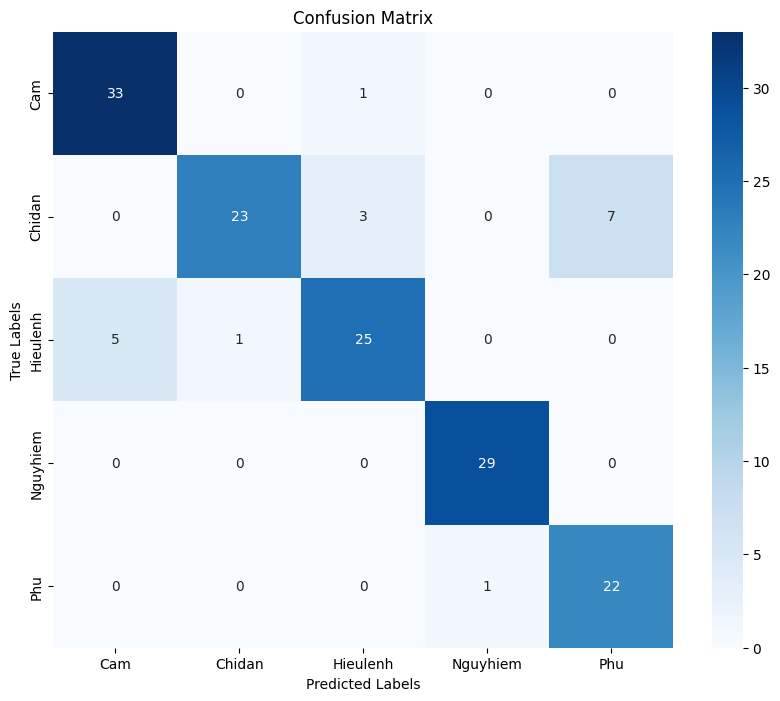
\includegraphics[width=0.7\textwidth]{knn_result_heatmap.png}
    \caption{Confusion Matrix của mô hình KNN}
    \label{fig:knn_confusion_matrix}
\end{figure}

\paragraph{SVM}  
Kết quả dự đoán của mô hình SVM được tóm tắt như sau:
\begin{itemize}
    \item \textbf{Nhóm \textit{Cấm}}: Dự đoán đúng 32 biển báo. Chỉ có 2 biển bị phân loại sai, tương tự như hiệu suất khi sử dụng mô hình KNN để phân loại. Điều này cho thấy SVM phân biệt rất tốt nhóm \textit{Cấm}.
    \item \textbf{Nhóm \textit{Chỉ dẫn}}: Dự đoán đúng 30 biển báo. Tuy nhiên, có 1 biển bị nhầm với nhóm \textit{Hiệu lệnh} và 2 biển nhầm với nhóm \textit{Phụ}. Điều này phản ánh sự cải thiện so với KNN.
    \item \textbf{Nhóm \textit{Hiệu lệnh}}: Dự đoán đúng 24 biển báo. Có 1 biển nhầm với nhóm \textit{Phụ}, 2 biển nhầm với nhóm \textit{Cấm} và 4 biển nhầm với nhóm \textit{Chỉ dẫn}, phản ánh rằng các chi tiết phức tạp trong nhóm này vẫn là một thách thức đối với mô hình.
    \item \textbf{Nhóm \textit{Nguy hiểm}}: Dự đoán đúng toàn bộ 29 biển báo mà không có bất kỳ sự nhầm lẫn nào. Điều này cho thấy SVM nhận diện xuất sắc các đặc trưng nổi bật của nhóm \textit{Nguy hiểm}.
    \item \textbf{Nhóm \textit{Phụ}}: Dự đoán đúng 20 biển báo. Có 1 biển bị nhầm lẫn với nhóm \textit{Hiệu lệnh} và 2 biển nhầm với nhóm \textit{Chỉ dẫn}. Điều này cho thấy hiệu suất của SVM ở nhóm này vẫn còn hạn chế và có hiệu suất tệ hơn KNN.
\end{itemize}

\textbf{Nhận xét}:  
Mô hình SVM cải thiện đáng kể so với KNN ở nhóm \textit{Chỉ dẫn}, với số lượng biển báo được dự đoán đúng tăng lên đáng kể. Nhóm \textit{Nguy hiểm} và \textit{Cấm} tiếp tục đạt hiệu suất tối đa, không có nhầm lẫn. Tuy nhiên, nhóm \textit{Hiệu lệnh} vẫn gây khó khăn cho mô hình, với các biển báo bị nhầm lẫn với các nhóm \textit{Cấm}, \textit{Chỉ dẫn} và \textit{Phụ}. Điều này cho thấy cần tập trung vào việc cải thiện khả năng phân biệt chi tiết phức tạp và tương đồng giữa các nhóm này. Đặc biệt khi sử dụng mô hình SVM để phân loại biển \textit{Phụ} thì có hiệu suất giảm đi so với khi sử dụng mô hình KNN.

\begin{figure}[H]
    \centering
    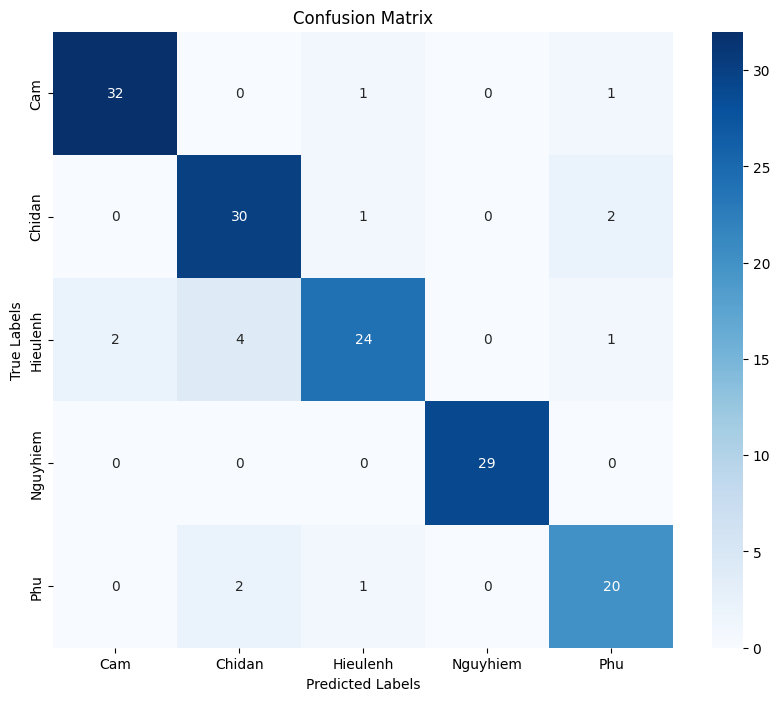
\includegraphics[width=0.7\textwidth]{svm_result_heatmap.png}
    \caption{Confusion Matrix của mô hình SVM}
    \label{fig:svm_confusion_matrix}
\end{figure}

\subsubsection{Nhận xét về kết quả}

\textbf{\textit{Classification report}} cung cấp thông tin chi tiết về các chỉ số như \textit{precision}, \textit{recall}, và \textit{F1-score} cho từng nhóm biển báo, qua đó đánh giá hiệu suất toàn diện của mô hình KNN. Đây là một công cụ quan trọng để hiểu rõ hơn về những điểm mạnh và hạn chế trong khả năng phân loại của mô hình trên từng loại biển báo cụ thể.  

\paragraph{KNN}  
Mô hình KNN đạt độ chính xác tổng thể (\textit{accuracy}) ở mức 88\%, thể hiện khả năng phân loại tốt trên tập dữ liệu kiểm tra. Tuy nhiên, các chỉ số hiệu suất của từng nhóm biển báo cho thấy sự khác biệt đáng kể:  
\begin{itemize}
    \item \textbf{Nhóm \textit{Cấm}}: Đạt hiệu suất cao nhất với \textit{recall} là 97\% và \textit{F1-score} là 92\%. Mô hình nhận diện rất tốt các biển báo thuộc nhóm này nhờ đặc trưng hình học và màu sắc nổi bật, giúp dễ dàng phân biệt với các nhóm khác.  
    \item \textbf{Nhóm \textit{Chỉ dẫn}}: Mặc dù có \textit{precision} cao (96\%), \textit{recall} chỉ đạt 70\%, dẫn đến \textit{F1-score} là 81\%. Điều này cho thấy mô hình dễ bỏ sót các biển báo thuộc nhóm này, đặc biệt là những biển báo có nhiều chi tiết hoặc tương đồng với các nhóm khác.  
    \item \textbf{Nhóm \textit{Hiệu lệnh}}: Hiệu suất khá tốt với \textit{F1-score} là 83\%. Tuy nhiên, mô hình vẫn gặp khó khăn trong việc phân biệt nhóm này với các nhóm khác do chi tiết phức tạp hoặc sự tương đồng giữa các biển báo, chẳng hạn như về màu sắc hoặc hình dạng.  
    \item \textbf{Nhóm \textit{Nguy hiểm}}: Đây là nhóm được phân loại tốt nhất, đạt cả \textit{recall} và \textit{precision} rất cao, lần lượt là 100\% và 97\%. Điều này cho thấy mô hình phát hiện chính xác hầu hết các biển báo thuộc nhóm này nhờ vào đặc điểm viền đỏ tam giác rất dễ nhận biết.  
    \item \textbf{Nhóm \textit{Phụ}}: Hiệu suất khá tốt với \textit{recall} là 96\% và \textit{F1-score} là 85\%. Tuy nhiên, \textit{precision} chỉ đạt 76\%, phản ánh sự nhầm lẫn giữa nhóm này và các nhóm khác, đặc biệt là những biển báo có kích thước nhỏ hoặc ít nổi bật trong hình ảnh.  
\end{itemize}

Nhìn chung, KNN hoạt động tốt với các nhóm biển báo có đặc trưng hình học và màu sắc nổi bật như \textit{Cấm} và \textit{Nguy hiểm}. Tuy nhiên, các nhóm như \textit{Chỉ dẫn}, \textit{Hiệu lệnh}, và \textit{Phụ} vẫn gây khó khăn do đặc điểm phức tạp hoặc sự tương đồng giữa các nhóm, dẫn đến tỷ lệ bỏ sót và nhầm lẫn đáng kể.

\begin{figure}[H]
    \centering
    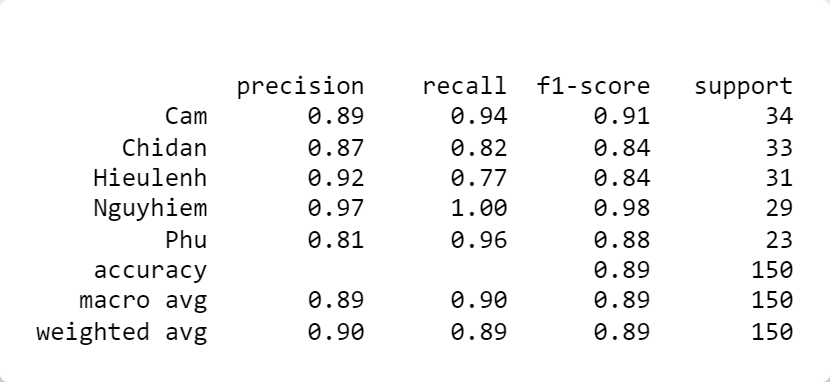
\includegraphics[width=0.7\textwidth]{classification_report_knn.png}
    \caption{Classification Report của mô hình KNN}
    \label{fig:knn_classification_report}
\end{figure}

\paragraph{SVM}
Mô hình SVM đạt độ chính xác tổng thể (\textit{accuracy}) ở mức 91\%, vượt trội hơn so với KNN. Các chỉ số \textit{precision}, \textit{recall}, và \textit{F1-score} cho từng nhóm biển báo cũng thể hiện sự cải thiện đáng kể:
\begin{itemize} \item \textbf{Nhóm \textit{Cấm}}: Mô hình đạt \textit{recall} là 97\% và \textit{F1-score} là 93\%, cho thấy khả năng nhận diện khá tốt đối với nhóm này.
\item \textbf{Nhóm \textit{Chỉ dẫn}}: Cải thiện rõ rệt với cả \textit{precision} và \textit{recall} đạt 88\%, dẫn đến \textit{F1-score} là 88\%. Điều này thể hiện rằng SVM giảm đáng kể tỷ lệ bỏ sót so với KNN.
\item \textbf{Nhóm \textit{Hiệu lệnh}}: Mặc dù \textit{precision} cao (92\%), \textit{recall} chỉ đạt 77\%, dẫn đến \textit{F1-score} là 84\%. Nhóm này vẫn là thách thức với SVM do đặc trưng phức tạp của các biển báo.
\item \textbf{Nhóm \textit{Nguy hiểm}}: Hiệu suất rất cao, với \textit{recall} đạt 100\% và \textit{F1-score} là 98\%, tương tự KNN. Mô hình phân loại chính xác hầu hết các biển báo thuộc nhóm này.
\item \textbf{Nhóm \textit{Phụ}}: Với \textit{recall} là 91\% và \textit{F1-score} là 89\%, nhóm này đạt hiệu suất cao hơn KNN, cho thấy khả năng phân biệt của SVM tốt hơn đối với nhóm có đặc điểm ít rõ ràng hơn.
\end{itemize}

Nhìn chung, SVM vượt trội hơn KNN trong việc nhận diện các nhóm biển báo phức tạp như \textit{Chỉ dẫn} và \textit{Phụ}, nhờ vào khả năng tối ưu hóa siêu phẳng phân tách. Tuy nhiên, nhóm \textit{Hiệu lệnh} vẫn gây khó khăn cho mô hình do sự đa dạng trong đặc trưng biển báo.

\begin{figure}[H]
    \centering
    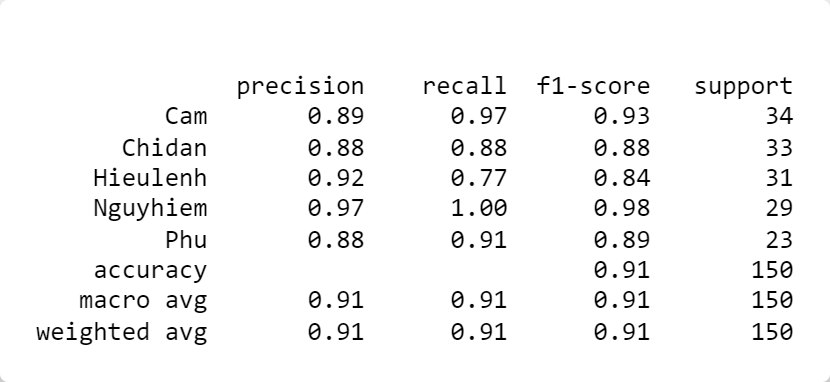
\includegraphics[width=0.7\textwidth]{classification_report_svm.png}
    \caption{Classification Report của mô hình SVM}
    \label{fig:svm_classification_report}
\end{figure}

\newpage
\subsection{Minh họa các ảnh phân loại}

\subsubsection{Ảnh từ tập test}

Dưới đây là các ảnh từ tập kiểm tra, được phân loại bởi các mô hình KNN và SVM.

\begin{figure}[H]
    \centering
    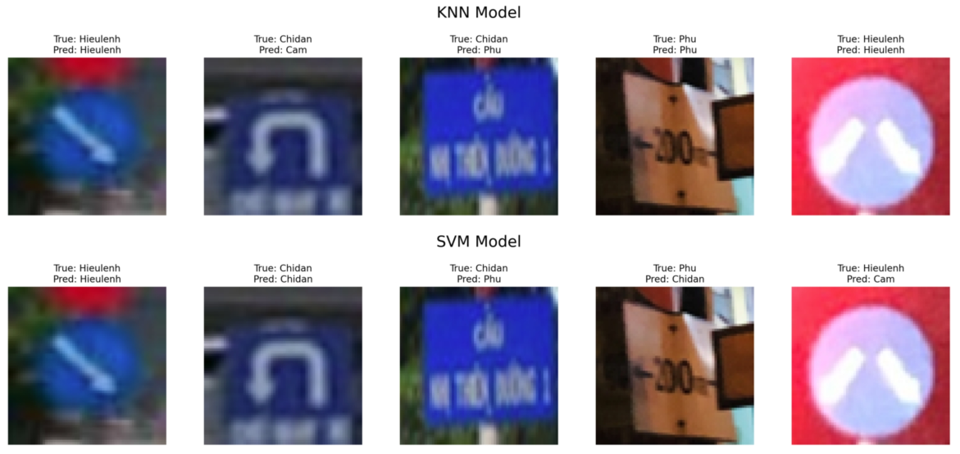
\includegraphics[width=0.95\textwidth]{demo_test_images.png}
    \caption{Ảnh từ tập test}
    \label{fig:test_images}
\end{figure}

\subsubsection{Ảnh không tồn tại trong bộ dữ liệu}

Các ảnh dưới đây không tồn tại trong bộ dữ liệu huấn luyện và kiểm tra, và được phân loại bởi các mô hình KNN và SVM.

\begin{figure}[H]
    \centering
    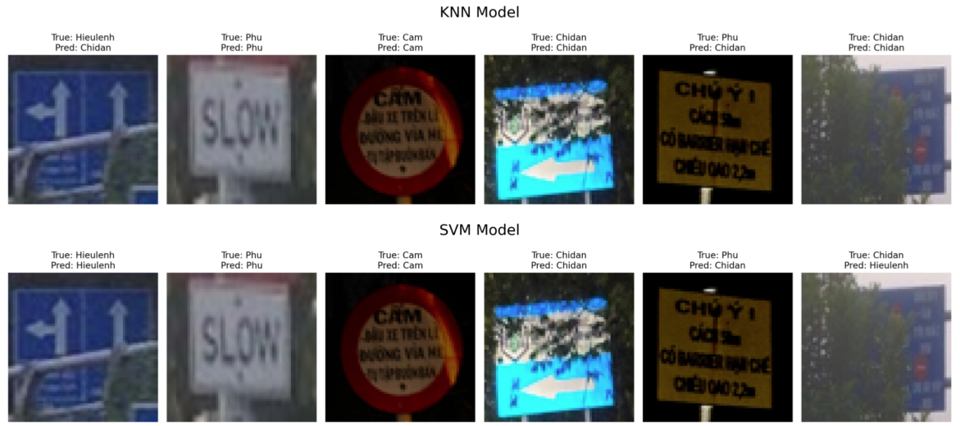
\includegraphics[width=0.95\textwidth]{demo_new_images.png}
    \caption{Ảnh không tồn tại trong bộ dữ liệu}
    \label{fig:new_images}
\end{figure}

\newpage
\section*{\centering Web Demo Phân Loại Biển Báo Giao Thông}
\addcontentsline{toc}{section}{\textbf{WEB DEMO PHÂN LOẠI BIỂN BÁO GIAO THÔNG}}
\vspace{1cm}
\setcounter{section}{4}
\setcounter{subsection}{0}

\subsection{Giới thiệu}
\hspace{5mm}Web demo này được xây dựng để phân loại biển báo giao thông sử dụng hai mô hình học máy: KNN (K-Nearest Neighbors) và SVM (Support Vector Machine).

\subsection{Cách sử dụng}
\subsubsection{Chọn mô hình}
\begin{itemize}
    \item Người dùng có thể chọn sử dụng mô hình tốt nhất (Best Model) hoặc tùy chỉnh thông số.
    \item Đối với KNN: có thể điều chỉnh n\_neighbors, weights và metrics
    \item Đối với SVM: có thể điều chỉnh kernel, C, degree và gamma
\end{itemize}

\subsubsection{Xem kết quả đánh giá}
\begin{itemize}
    \item Classification Report: hiển thị các metric đánh giá (precision, recall, f1-score)
    \item Confusion Matrix: thể hiện kết quả phân loại 1 cách chi tiết
\end{itemize}

\subsubsection{Phần Demo}
\begin{itemize}
    \item Xem kết quả phân loại trên ảnh từ tập test
    \item Xem kết quả phân loại trên ảnh mới (không có trong tập dữ liệu)
\end{itemize}

\subsubsection{Thử nghiệm}
\begin{itemize}
    \item Người dùng có thể tải lên ảnh biển báo của riêng mình (hỗ trợ nhiều định dạng ảnh: jpg, jpeg, png)
    \item Hệ thống sẽ hiển thị kết quả phân loại từ cả hai mô hình
\end{itemize}

\subsection{Truy cập web}
\hspace{5mm}Để truy cập trang web, nhấn vào \href{https://traffic-sign-classification-through-images.streamlit.app/}{\textbf{Traffic Sign Classification Web}} hoặc quét mã QR dưới đây:
\begin{center}
    
\includegraphics[width=0.3\textwidth]{link_web.png}
\end{center}

\newpage
\pagenumbering{gobble}
\thispagestyle{empty}
\addcontentsline{toc}{section}{\protect\numberline{}KẾT LUẬN}
% \hrule height 0.4pt
\begin{center}
    \textbf{\large KẾT LUẬN}
\end{center}
\vspace{1cm}
\subsection*{Kết luận chung}

\hspace{6mm}- Với tập dataset đã được chuẩn bị, trong hai mô hình mà nhóm chọn, mô hình \textbf{SVM} đạt độ chính xác cao nhất với \textbf{91\%}. Mô hình này cho thấy khả năng phân loại tốt đối với hầu hết các nhóm biển báo. 

- Nhóm \textit{Cấm} được phân loại tốt nhất trên cả hai mô hình, với độ chính xác cao. Nguyên nhân có thể do số lượng ảnh của nhóm \textit{Cấm} cao hơn so với các nhóm khác, và đặc trưng của biển báo \textit{Cấm} (thường có viền và nền màu đỏ) giúp mô hình dễ dàng nhận diện nhờ sự khác biệt màu sắc mạnh mẽ, ít bị nhầm lẫn với các biển báo khác.
  
- Nhóm \textit{Hiệu lệnh}, \textit{Chỉ dẫn} và \textit{Phụ} thường bị nhầm lẫn do màu sắc, hình dạng có phần tương đồng kèm theo nội dung chi tiết trong biển báo là quá nhiều. Điều này thể hiện sự cần thiết phải cải thiện khả năng phân biệt chi tiết giữa các biển báo này.

- Điều kiện môi trường có thể gây khó khăn cho việc nhận diện biển báo, chẳng hạn như khi biển báo bị che khuất bởi ánh sáng yếu, thời tiết xấu như mưa hoặc sương mù, hoặc khi hình ảnh có chất lượng kém. Những yếu tố này ảnh hưởng đến khả năng quan sát và phân loại chính xác của mô hình.

\subsection*{Hướng phát triển}

\hspace{6mm}- \textbf{Mở rộng và cải thiện dataset:}
    \begin{itemize}
        \item Thu thập thêm dữ liệu, đặc biệt là những biển báo trong các điều kiện môi trường khác nhau (ánh sáng yếu, mưa, sương mù, các góc chụp khác nhau) để tăng tính đa dạng và khả năng tổng quát hóa của mô hình.
        \item Sử dụng dữ liệu từ nhiều nguồn khác nhau, bao gồm cả hình ảnh từ các camera khác nhau, để cải thiện độ chính xác và tính tổng quát của mô hình.
    \end{itemize}

- \textbf{Cải thiện tiền xử lý dữ liệu:}
    \begin{itemize}
        \item Áp dụng các kỹ thuật tiền xử lý như cân bằng sáng và tăng cường ảnh để cải thiện chất lượng hình ảnh đầu vào.
        \item Phát hiện và loại bỏ nhiễu trong hình ảnh nhằm nâng cao độ chính xác của mô hình.
    \end{itemize}

- \textbf{Nâng cấp mô hình phân loại:}
    \begin{itemize}
        \item Triển khai các mô hình học sâu để cải thiện khả năng nhận diện và phân loại biển báo giao thông.
    \end{itemize}

- \textbf{Cải thiện đặc trưng trích xuất:}
    \begin{itemize}
        \item Kết hợp nhiều phương pháp trích xuất đặc trưng để tăng cường độ chính xác và khả năng phân loại của mô hình.
    \end{itemize}

\newpage
\thispagestyle{empty}
\addcontentsline{toc}{section}{\protect\numberline{}TÀI LIỆU THAM KHẢO}
\begin{center}
    \textbf{\large TÀI LIỆU THAM KHẢO}
\end{center}
\vspace{1cm}
\sloppy
\printbibliography

\end{document}
